\subsection{Motivation}
Motivation of the model we studied can be found in the IP-based computer networks 
problems. Router has to store enormous number of forwarding rule and this number is 
still growing. The fast router memory is expensive and requires a lot of energy, 
which is a big problem for Internet Service Providers. As a solution to this 
problem there comes Software-Defined Networking (SDN) technology. It consists of two 
types of memory: the fast memory, which is kept in router and the slow one, which is 
placed in so called controller. The latter one keeps information about all of the FIB rules. 
On the other hand, router keeps only the part of the FIB tree. Whenever a packet comes, it is firstly 
processed by the router. If its forwarding rule is found in the router's cache, then it 
is immediately forwarded to its final destination. In the case of not finding the appropriate
rule for the packet, we fetch that rule from the slow memory paying $1$ for each such request. At some points of 
time the controller may decide to change the router's cache by inserting or deleting 
a rule. Any such operation costs us $\alpha$. Figure \ref{fig:motivation} shows 
the crucial concepts, that were just briefly described. More detailed and 
technical description can found in \cite{sdn}.
 \begin{figure}
 \begin{center}
  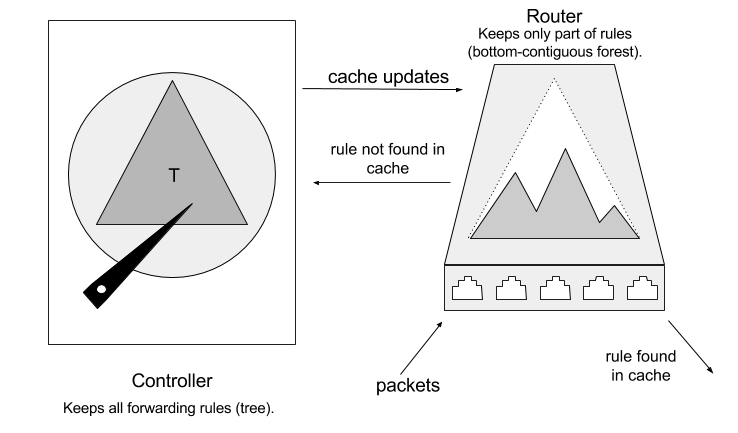
\includegraphics[width=0.8\textwidth]{motivation.png}
\end{center}
\caption{}
\label{fig:motivation}
\end{figure}

The tree caching model can be easily applied, fitting to the SND architecture 
assumptions. Fast memory here is obviously router's cache and the 
controller maps to slow memory of the tree caching problem. Positive requests 
correspond to looking up forwarding rules for a given packet. Whenever we want to evict an item from 
router's cache, we can send $\alpha$ negative requests in our model to trigger 
the eviction. Whats is more, the tree structure and bottom-contiguity arise 
from the FIB's longest matching prefix scheme (LMP). Precisely, when we are given a 
packet, we search for forwarding rule, which matches the longest prefix with the 
IP destination of packet. The IP addresses form a tree like 
structure in its nature, where the most general rule is placed in the root and in the leaves 
there are placed most precise rules. Notice, that if the router's cache was not 
bottom-contiguous, we might have faced a situation, where we would send packet to a
wrong destination, thus finding less specific rule. The bottom-contiguity assures then, that when the rule 
for the packet is found in the cache, it is similar to the most precise rule in the
controller.
